\hypertarget{manger-au-liban}{%
\section{Manger au Liban}\label{manger-au-liban}}

Comme je l'ai déjà écrit dans le premier billet sur le Liban, nous avons
été accueilli de manière extrêmement généreuse par la famille d'Elida.
Tout le monde s'occupe de nous, nous propose des excursions, demande
comment je trouve le Liban et... nous invite à manger. Cela se traduit
principalement par deux choses : la commande d'un nombre extraordinaire
de plats, bien au-delà du raisonnable, et le fait qu'on ressort de table
après plusieures heures en n'ayant plus du tout faim :D

\begin{figure}
\centering
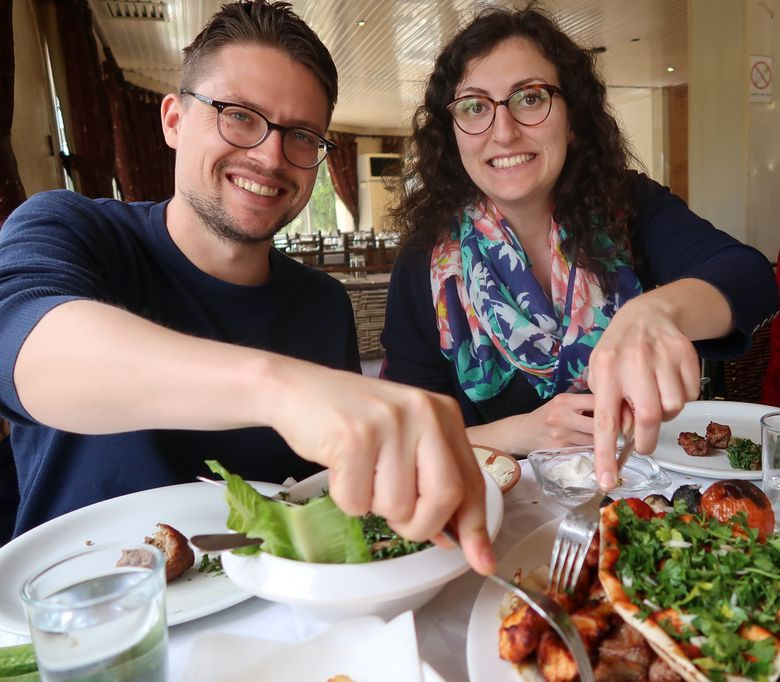
\includegraphics{images/20180523_manger.JPG}
\caption{Exemple de festin sur fond de gastronomes heureux.}
\end{figure}

Le déroulement d'un repas peut être décrit par la séquence suivante :

\begin{itemize}
\tightlist
\item
  on amène des petites choses à grignoter à la table (par exemple :
  olives, amandes vertes qu'on mange en entier, petits pois,
  cacahouètes)
\item
  le serveur demande "Fattoush ou Tabbouleh ?" et prend la commande des
  mezzés et des plats
\item
  le serveur sert le Fattoush / Tabbouleh, puis les mezzés arrivent et
  on en mange avec du pain libanais qu'on déchire pour former des petits
  récipients pour aller "pêcher" du Hommous et du Labneh
\item
  on n'a plus faim car tout est très bon et on a eu envie de tout goûter
\item
  les grillades (kefta, taouk de poulet, brochettes de boeuf) arrivent,
  on est surpris car on ne s'y attendait plus, et on en mange même si on
  a plus faim
\item
  on n'a vraiment plus faim
\item
  on passe au dessert (fruits frais, gâteau d'anniversaire ou de baptême
  s'il y a lieu, gâteaux pleins de sirop de sucre)
\end{itemize}

Optionnellement, on peut bien entendu commander un narguilé (qu'on
appelle d'ailleurs arguilé ici) que l'on "déguste" au fil du repas.

On peut noter que par rapport au repas français traditionnel, le repas
libanais ne s'accompagne pas forcément d'un café à la fin (je me suis
rendu compte qu'on sert le café "à la turque" à n'importe quelle heure
de la journée, et qu'il est généralement moins fort que le café que l'on
a coutume de boire en France).

Concernant les boissons alcoolisées, l'Arak occupe une place de premier
choix sur la table libanaise. Qu'il soit fait maison ou pas, on en
rencontre bien plus souvent que le vin de nos contrées.

Vous l'aurez compris, on mange bien au Liban.

Malheureusement, ceci m'amène au revers de la médaille : au restaurant,
ce qui est commandé mais n'a pas pu être mangé par les convives finit...
à la poubelle ! La culture de l'hospitalité prescrit un festin, mais ne
prévoit pas (encore ?) de garder les restes et de les ramener à la
maison.

Allez, on vous laisse saliver avec nos photos de repas libanais !

\emph{Florian}
